% This is the Reed College LaTeX thesis template. Most of the work 
% for the document class was done by Sam Noble (SN), as well as this
% template. Later comments etc. by Ben Salzberg (BTS). Additional
% restructuring and APA support by Jess Youngberg (JY).
% Your comments and suggestions are more than welcome; please email
% them to cus@reed.edu
%
% See http://web.reed.edu/cis/help/latex.html for help. There are a 
% great bunch of help pages there, with notes on
% getting started, bibtex, etc. Go there and read it if you're not
% already familiar with LaTeX.
%
% Any line that starts with a percent symbol is a comment. 
% They won't show up in the document, and are useful for notes 
% to yourself and explaining commands. 
% Commenting also removes a line from the document; 
% very handy for troubleshooting problems. -BTS

% As far as I know, this follows the requirements laid out in 
% the 2002-2003 Senior Handbook. Ask a librarian to check the 
% document before binding. -SN

%%
%% Preamble
%%
% \documentclass{<something>} must begin each LaTeX document
\documentclass[12pt,twoside]{reedthesis}
% Packages are extensions to the basic LaTeX functions. Whatever you
% want to typeset, there is probably a package out there for it.
% Chemistry (chemtex), screenplays, you name it.
% Check out CTAN to see: http://www.ctan.org/
%%
\usepackage{graphicx,latexsym} 
\usepackage{amssymb,amsthm,amsmath}
\usepackage{longtable,booktabs,setspace} 
\usepackage{chemarr} %% Useful for one reaction arrow, useless if you're not a chem major
\usepackage[hyphens]{url}
\usepackage{rotating}
\usepackage{natbib}
\usepackage{ifthen}
\usepackage{color}
\graphicspath{{./Figs/}} % Set graphics path
% Comment out the natbib line above and uncomment the following two lines to use the new 
% biblatex-chicago style, for Chicago A. Also make some changes at the end where the 
% bibliography is included. 
%\usepackage{biblatex-chicago}
%\bibliography{thesis}

% \usepackage{times} % other fonts are available like times, bookman, charter, palatino


%%%% REFERENCES %%%%%
\newcommand{\rf}     [1] {~\cite{#1}}
\newcommand{\refref} [1] {ref.~\cite{#1}}
\newcommand{\refRef} [1] {Ref.~\cite{#1}}
\newcommand{\refrefs}[1] {refs.~\cite{#1}}
\newcommand{\refRefs}[1] {Refs.~\cite{#1}}
\newcommand{\refeq}  [1] {Eq.~(\ref{#1})}
\newcommand{\refeqs} [2]{Eqs.~\ref{#1} and \ref{#2}}
\newcommand{\refFig} [1] {Fig.~\ref{#1}}
\newcommand{\refFigs} [2] {Figs.~\ref{#1} and~\ref{#2}}
\newcommand{\reftab} [1] {Table~\ref{#1}}
\newcommand{\refTab} [1] {Table~\ref{#1}}
\newcommand{\reftabs}[2] {tables~\ref{#1} and~\ref{#2}}
\newcommand{\refsect}[1] {Section~\ref{#1}}
\newcommand{\refsects}[2] {Sections~\ref{#1} and \ref{#2}}
\newcommand{\refSect}[1] {Section~\ref{#1}}
\newcommand{\refSects}[2] {Sects.~\ref{#1} and \ref{#2}}
\newcommand{\refsecttosect}[2] {Sects.~\ref{#1} to~\ref{#2}}
\newcommand{\refappe}[1] {appendix~\ref{#1}}
\newcommand{\refappes}[2] {appendices~\ref{#1} and~\ref{#2}}
\newcommand{\refAppe}[1] {Appendix~\ref{#1}}
\newcommand{\refChapter}[1]{Chapter~\ref{#1}}
\newcommand{\refChapt}[1]{Chapt.~\ref{#1}}
\newcommand{\ignore}[1]{}
\newcommand{\nobibentry}[1]{{\let\nocite\ignore\bibentry{#1}}}
\newcommand{\bibfnamefont}[1]{#1}
\newcommand{\bibnamefont}[1]{#1}


%%%% SYMBOLS %%%%
\newcommand{\ReN}{\ensuremath{Re}} % Reynolds number

%%%% ABBREVIATIONS %%%%%
\newcommand{\etc}{{etc.}}       % APS
\newcommand{\etal}{{\em et al.}}    % etal in italics, APS too
\newcommand{\ie}{{i.e.}}        % APS
\newcommand{\cf}{{\em cf.\ }}     % APS
\newcommand{\eg}{{e.g.\ }}        % APS, OUP, hard space '\eg\ NextWord'

%%%%% EDITING COMMANDS %%%%%
\newcommand{\DB}[2]{$\footnotemark\footnotetext{DB #1: {\color{red}#2}}$} %date, comment
\newcommand{\DBedit}[1]{{\color{red}#1}}
\newcommand{\MC}[2]{$\footnotemark\footnotetext{DB #1: {\color{green}#2}}$} %date, comment
\newcommand{\MCedit}[1]{{\color{green}#1}}
 % Load thesis specific macros

\title{My Final College Paper}
\author{Your R. Name}
% The month and year that you submit your FINAL draft TO THE LIBRARY (May or December)
\date{May 200x}
\division{Mathematics and Natural Sciences}
\advisor{Advisor F. Name}
%If you have two advisors for some reason, you can use the following
%\altadvisor{Your Other Advisor}
%%% Remember to use the correct department!
\department{Mathematics}
% if you're writing a thesis in an interdisciplinary major,
% uncomment the line below and change the text as appropriate.
% check the Senior Handbook if unsure.
%\thedivisionof{The Established Interdisciplinary Committee for}
% if you want the approval page to say "Approved for the Committee",
% uncomment the next line
%\approvedforthe{Committee}

\setlength{\parskip}{0pt}
%%
%% End Preamble
%%
%% The fun begins:
\begin{document}

  \maketitle
  \frontmatter % this stuff will be roman-numbered
  \pagestyle{empty} % this removes page numbers from the frontmatter

% Acknowledgements (Acceptable American spelling) are optional
% So are Acknowledgments (proper English spelling)
%	% Acknowledgements (Acceptable American spelling) are optional
% So are Acknowledgments (proper English spelling)
    \chapter*{Acknowledgements}
	I want to thank a few people.
	
	%Help with thesis
	%Daniel, Jay, Bob. Kai, Lily, jack for reading drafts. daniel
	
	%Physics profs
	%Daniel, Darrell, Nelia, johnny, Joel, Lucas
	
	%Other profs
	% Albert, Libby, Alan (sp?), 
	
	% Parents
	
	% Kai
	
	% Lily and Clops
	
	

% The preface is optional
% To remove it, comment it out or delete it.
%	% The preface is optional
% To remove it, comment it out or delete it.
    \chapter*{Preface}
	This is an example of a thesis setup to use the reed thesis document class.

%  \tableofcontents
% if you want a list of tables, optional
%  \listoftables
% if you want a list of figures, also optional
%  \listoffigures
		
% The abstract is not required if you're writing a creative thesis (but aren't they all?)
% If your abstract is longer than a page, there may be a formatting issue.
%	% The abstract is not required if you're writing a creative thesis (but aren't they all?)
% If your abstract is longer than a page, there may be a formatting issue.
    \chapter*{Abstract}
	In 2005 Yves Couder's group discovered that and oil droplet placed on a vibrating bath of the same oil would bounce along the surface of the oil indefinitely, propelled by the waves it created \rf{Couder2005a}. This ``walker" exhibits many behaviors analogous to those observed in quantum systems, such as single particle double slit diffraction \rf{double-slit}, quantized orbits \rf{Oza2014}, and among others \rf{pilot-wave}, tunneling \rf{tunneling}. Tunneling occurs when a droplet interacts with a subsurface barrier; the droplet either passes over or reflects off of the barrier. In experiments described here, we studied the dependence of the tunneling probability on the height of a barrier of width $e=3.0~\mathrm{mm}$. It was determined that tunneling occurred for depths $h>1.0~\mathrm{mm}$, and appeared probabilistic at an oil depth of $h=1.25~\mathrm{mm}$. It was also observed that droplets with higher momentum are more likely to tunnel. 
%		\chapter*{Dedication}
	You can have a dedication here if you wish.

  \mainmatter % here the regular arabic numbering starts
  \pagestyle{fancyplain} % turns page numbering back on

% Double spacing: if you want to double space, or one and a half 
% space, uncomment one of the following lines. You can go back to 
% single spacing with the \singlespacing command.
% \onehalfspacing
% \doublespacing

%	%The \introduction command is provided as a convenience.
%if you want special chapter formatting, you'll probably want to avoid using it altogether
		
\chapter*{Introduction}
    \addcontentsline{toc}{chapter}{Introduction}
		\chaptermark{Introduction}
		\markboth{Introduction}{Introduction}
% The three lines above are to make sure that the headers are right, that the intro gets included in the table of contents, and that it doesn't get numbered 1 so that chapter one is 1.





	(Important: Particle-wave association on a fluid interface (Protiere 2006)).
	    
	    In 2005, Yves Couder showed that bouncing oil drops on vertically vibrating fluid bath exhibited properties analogous to the paradoxical properties seen only at the quantum scale (CITE: Dynamical phenomena:  Walking and orbiting droplets?). Couder, John Bush, and others have shown that this system can reproduce double-slit single-particle interference, orbiting, tunneling, quantized orbits, spin, and more.

	    	    \subsection{Faraday Waves}
	    
	    
	?

	    
	    \subsection{Bouncing Droplets}
	    Though it had been seen for at least a century, the phenomena of droplets bouncing on a fluid bath was first explained by Jearl Walker in 1978\rf{Walker}. The investigations began with a simple droplet of water falling onto a bath of water, and remaining just a second too long before coalescence.\footnote{I don't drink coffee so I haven't seen this, but everyone seems to cite that this occurrs with coffeemakers, as the coffee drips into the pot.} It was then discovered that adding detergent to the water and then vibrating the bath would extend the lifetime of these droplets from fractions of a second to several minutes. Because these droplets are bouncing at frequencies of around 50 Hz (50 bounces per second) and the droplets are very small to begin with (with a diameter of a millimeter or less), it can be difficult to observe even the main mechanisms that drive the behaviour. A key insight by Walker was to flash a strobelight at a frequency slightly slower than the rate of vibration of the fluid bath, that way he could observe the droplet bouncing as if in slow motion.
	    
	    Walker found that a trapped film of air kept the droplet and the bath from touching, as shown in \refFig{bounce}. That is, the droplet is bouncing on a layer of air that's struggling to get out of the way but because the bounce happens so quickly, the fluid droplet and the fluid bath never touch. Walker concluded that the leakage rate of this trapped pocket of air depends on three factors: the nature of surface tension of the fluid bath, the viscosity of the droplet and the fluid bath, and the viscocity of the air. The bath must be of uniform surface tension and free from particulate matter floating atop the bath, since both will lead to coalescence. Higher viscosity fluids translate to longer droplet lifetimes, since more viscous fluids keep air from escaping the pocket. Finally, adjusting the frequency and the amplitudes of the vibrations also affects droplet lifetime.\footnote{Reedie Andrew Case ('92) wrote his thesis ``Oil on Troubled Water: The Extension of Floating Drop Lifetimes Due to Interface Vibration" where he looked at droplet lifetime by the frequency of vibration.}   
	     
	    More recent research suggests that a droplet fluid like silicone oil could bounce indefinately of a vibrating bath\rf{Couder2005a}. The long lifetime occurs not only because silicone oil has a high viscosity, but also because it has a \textit{low} surface tension. A low surface tension is beneficial because it makes the oil bath relatively immune to surfactants (surface acting agents) or contaminations which would otherwise make the surface tension nonuniform, and thus create a coalescence event. 
	    
	    
	    
	    	    
	   	        
	    %(NONCOALESCENCE AND NONWETTING BEHAVIOR OF LIQUIDS
%Annual Review of Fluid Mechanics
%Vol. 34: 267-289 (Volume publication date January 2002)
%DOI: 10.1146/annurev.fluid.34.082701.154240
%G. Paul Neitzel1 and Pasquale Dell'Aversana2
%)

	    
	 
	    
	    	    \subsection{Walking Droplets}
	    
	       It was Couder who then showed that an oil droplet could live for much longer. Long lifetimes meant that the focus could shift from how the doplet bounced (short time scale) to its interactions with other droplets and its motion (longer time scale).
	       
	       Every time the droplet impacts the bath, it creates a radial traveling wave. If the bouncing droplet impacts the wavefield in such a way that it recives a lateral force from the slope of the wave, then it will be pushed to the side slightly. The next time the droplet makes contanct with the bath, it will again make contact with a slope, and be pushed to the side. This propels the bouncing droplet, causing it to ``walk" across the surface of the bath. These ``walkers" turned out to have particularly interesting behaviours. Indeed, in 2006 Yves Couder and Emmanuel Fort showed that these droplets mimicked the behavior of electrons in the hallmark experiment of quantum weirdness: the double slit experiment. This was the first time that microscopic scale behavior had ever been seen at a macroscopic level, and it sparked interest in the experiment.
	    
	    
	
%	\chapter{The First}
    	This is the first \ReN\ page of the first chapter. You may delete the contents of this chapter so you can add your own text; it's just here to show you some examples.\DB{9/30/2014}{What are you talking about?}
			
\section{References, Labels, Custom Commands and Footnotes}\label{Sect1}
It is easy to refer to anything within your document using the \texttt{label} and \texttt{ref} tags.  Labels must be unique and shouldn't use any odd characters; generally sticking to letters and numbers (no spaces) should be fine. Put the label on whatever you want to refer to, and put the reference where you want the reference. \LaTeX\ will keep track of the chapter, section, and figure or table numbers for you. 

\subsection{References and Labels}
Sometimes \MCedit{u'd like to refer to a table or figure, e.g. you can see in Figure \ref{subd2} that you can rotate figures .} Start by labeling your figure or table with the label command (\verb=\label{labelvariable}=) below the caption (see the chapter on graphics and tables for examples). Then when you would like to refer to the table or figure, use the ref command (\verb=\ref{labelvariable}=). Make sure your label variables are unique; you can't have two elements named ``default." Also, since the reference command only puts the figure or table number, you will have to put  ``Table" or ``Figure" as appropriate, as seen in the following examples:

 As I showed in Table \ref{inheritance} many factors can be assumed to follow from inheritance. Also see the Figure \ref{subd} for an illustration.
 
\subsection{Custom Commands}\label{commands}
Are you sick of writing the same complex equation or phrase over and over? 

The custom commands should be placed in the preamble, \refSect{Sect1} or at least prior to the first usage of the command. The structure of the \verb=\newcommand= consists of the name of the new command in curly braces, the number of arguments to be made in square brackets and then, inside a new set of curly braces, the command(s) that make up the new command. The whole thing is sandwiched inside a larger set of curly braces. 

% Note: you cannot use numbers in your commands!
\newcommand{\hydro}{H$_2$SO$_4$}

In other words, if you want to make a shorthand for H$_2$SO$_4$, which doesn't include an argument, you would write: \verb=\newcommand{\hydro}{H$_2$SO$_4$}= and then when you needed  to use the command you would type \verb=\hydro=. (sans verb and the equals sign brackets, if you're looking at the .tex version). For example: \hydro

\subsection{Footnotes and Endnotes}
	You might want to footnote something.\footnote{footnote text} Be sure to leave no spaces between the word immediately preceding the footnote command and the command itself. The footnote will be in a smaller font and placed appropriately. Endnotes work in much the same way. More information can be found about both on the CUS site.
	
\section{Bibliographies}
	Of course you will need to cite things, and you will probably accumulate an armful of sources. This is why BibTeX was created. For more information about BibTeX and bibliographies, see our CUS site (\url{web.reed.edu/cis/help/latex/index.html})\footnote{\cite{reedweb:2007}}. There are three pages on this topic: {\it bibtex} (which talks about using BibTeX, at \url{/latex/bibtex.html}), {\it bibtexstyles} (about how to find and use the bibliography style that best suits your needs, at \url{/latex/bibtexstyles.html}) and {\it bibman} (which covers how to make and maintain a bibliography by hand, without BibTeX, at at \url{/latex/bibman.html}). The last page will not be useful unless you have only a few sources. There used to be APA stuff here, but we don't need it since I've fixed this with my apa-good natbib style file.
	
\subsection{Tips for Bibliographies}
\begin{enumerate}
\item Like with thesis formatting, the sooner you start compiling your bibliography for something as large as thesis, the better. Typing in source after source is mind-numbing enough; do you really want to do it for hours on end in late April? Think of it as procrastination.
\item The cite key (a citation's label) needs to be unique from the other entries.
\item When you have more than one author or editor, you need to separate each author's name by the word ``and'' e.g.\\ \verb+Author = {Noble, Sam and Youngberg, Jessica},+.
\item Bibliographies made using BibTeX (whether manually or using a manager) accept LaTeX markup, so you can italicize and add symbols as necessary.
\item To force capitalization in an article title or where all lowercase is generally used, bracket the capital letter in curly braces.
\item You can add a Reed Thesis citation\footnote{\cite{noble:2002}} option. The best way to do this is to use the phdthesis type of citation, and use the optional ``type'' field to enter ``Reed thesis'' or ``Undergraduate thesis''. Here's a test of Chicago, showing the second cite in a row\footnote{\cite{noble:2002}} being different. Also the second time not in a row\footnote{\cite{reedweb:2007}} should be different. Of course in other styles they'll all look the same.
\end{enumerate}
\section{Anything else?}
If you'd like to see examples of other things in this template, please contact CUS (email cus@reed.edu) with your suggestions. We love to see people using \LaTeX\ for their theses, and are happy to help.

	\chapter{Introduction to Tunneling in QM}	


\section{Wavefunction}	
In classical mechanics, one can describe a particle with six variables: three position indicators ($x$, $y$, $z$), and three momentum indicators ($p_x$, $p_y$, $p_z$). One can find a function to represent variable by making multiple measurements across time, and discover an expression $x(t)$ that describes the particles location in space along the x dimension at time $t$. When all six variables can be described by a function, one can describe the position of the particle at any time.  

In quantum mechanics however, Heisenberg's uncertainty priciple limits the knowledge of position and momentum: 
$$\sigma_{x} \sigma_{p} \geq \hbar/2. $$
This equation states that as one knows more about the position of the system, then one loses knowledge about the momentum of the system, and vis versa. It's a tradeoff inherent to the nature of the system, not due to experimental deficiences. And it means that the strategy of finding equations for position and momentum of a system are no longer possible. If a particle has no exact position, can one represent where it might be? One can use a wave describing the probability of finding the particle at that position. The square root of this wave is called the wavefunction, and is represented by $\Psi(x, t)$.


\section{Schroedinger's Equation}

The wavefunction $\Psi(x, t)$ is goverened by the Schroedinger equation:

$$i\hbar\frac{\partial}{\partial t} \Psi(x,t) = \left [ \frac{-\hbar^2}{2m}\frac{\partial^2}{\partial x^2} + V(x,t)\right ] \Psi(x,t) $$
where $V(x,t)$ is the given potential, $m$ is the mass of the particle, and $\hbar$ is the reduced Planck's constant. For potentials that do not change in time, one can use separation of variables to arrive at the time-independant Schroedinger equation
$$E \Psi(x,t) = \left [ \frac{-\hbar^2}{2m}\frac{\partial^2}{\partial x^2} + V(x)\right ] \Psi(x,t)$$
where $E$ is the total energy. The goal is to find $\Psi(x,t)$ knowing the potential $V(x)$.




\section{Barrier Potential}

\section{Energies}
    \subsection{$E = V_0$}
    \subsection{$E > V_0$}
    \subsection{$E < V_0$}
    
    
    
    
\section{Physics}

Many of the symbols you will need can be found on the math page (\url{http://web.reed.edu/cis/help/latex/math.html}) and the Comprehensive \LaTeX\ Symbol Guide (enclosed in this template download).  You may wish to create custom commands for commonly used symbols, phrases or equations, as described in Chapter \ref{commands}.


	\chapter{Experimental Design}

In the our bouncing droplet system we observe surface waves guiding a droplet, and we're interested in learning more about the droplet-wave system in different settings. In this experiment, we will look at how features \textit{underneath} the surface of the oil (i.e. on the ``floor" of the tray) affect the motion of the droplet. 

A raised object on the floor of the tray (but still underneath the surface of the oil) can have an effect on height of the surface waves, and thus, on the motion of the walker. Sometimes a droplet headed towards a raised object will be reflected backwards, as if from a collision with the object. For this reason, we refer to a raised object as a barrier. Oftentimes however, the droplet continues on and crosses the barrier without a collision, this is analagous to ``transmission" the quantum mechanical process of tunneling. In other words, for a given barrier we will see a probability of tunneling unique to that barrier. Other studies have shown that increasing barrier width decreases probability of tunneling\rf{tunneling}. This study looks at how height of the barrier affects the tunneling probability. 

To test the effect of a barrier's height on the probability of tunneling, I used a combination of procedures from the investigations of Bush\rf{pilot-wave}, Couder\rf{Couder2005}, and specifically, Eddi et al.\rf{tunneling}. These were slightly modified to fit some of the unique features of my experiment. In this section I aim to give some of the reasoning behind the tray design and data collection techniques, both of which are not well described in the literature.

\section{Setup}
    The combined setup is shown in \refFig{setup}. A waveform generator creates a sinusoidal signal which is amplified and fed into a shaker. The shaker vibrates the tray vertically. Both the frequency and the amplitude of the vertical oscillations can be controlled. 
    
    An accelerometer records the vertical acceleration of the tray and is read by an oscilloscope. A camera records the droplet as it bounces along the surface of the oil.  
    
\begin{figure}[h!]
	\centering
	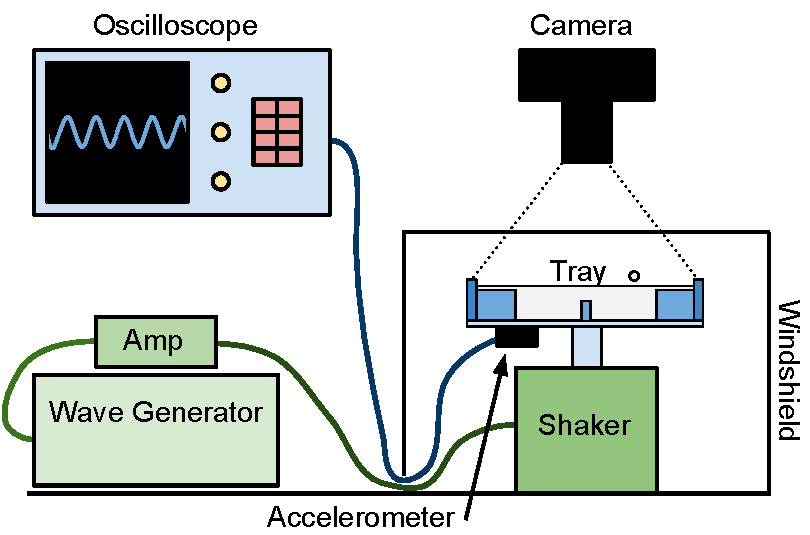
\includegraphics[scale=0.8]{Setup.pdf}
	\caption{The experimental setup. The amplified signal from the wave generator drives the shaker. The accelerometer generates a signal which is read by the oscilloscope. The shield blocks disturbances to the experiment, while allowing the camera to document the trials.}
	\label{setup}
\end{figure}

\section{Materials}
The key components of this experiment are the shaker, the oil, and the tray. In this section I'll describe the specifics of the holy trinity, as well as some of the additional components used in data collection. 

\subsection{Tray}
The tray was made of plastic parts machined by the (MODEL NUMBER?) laser cutter. They were then glued together with GLUE?. The tray's design, which was based off of the tray in the tunneling experiment done by Eddi et al.\rf{tunneling}, naturally guides the droplet into a perpendicular collision with the barrier. The tray schematic is shown in \refFig{tray}. 

\begin{figure}[h!]
	\centering
	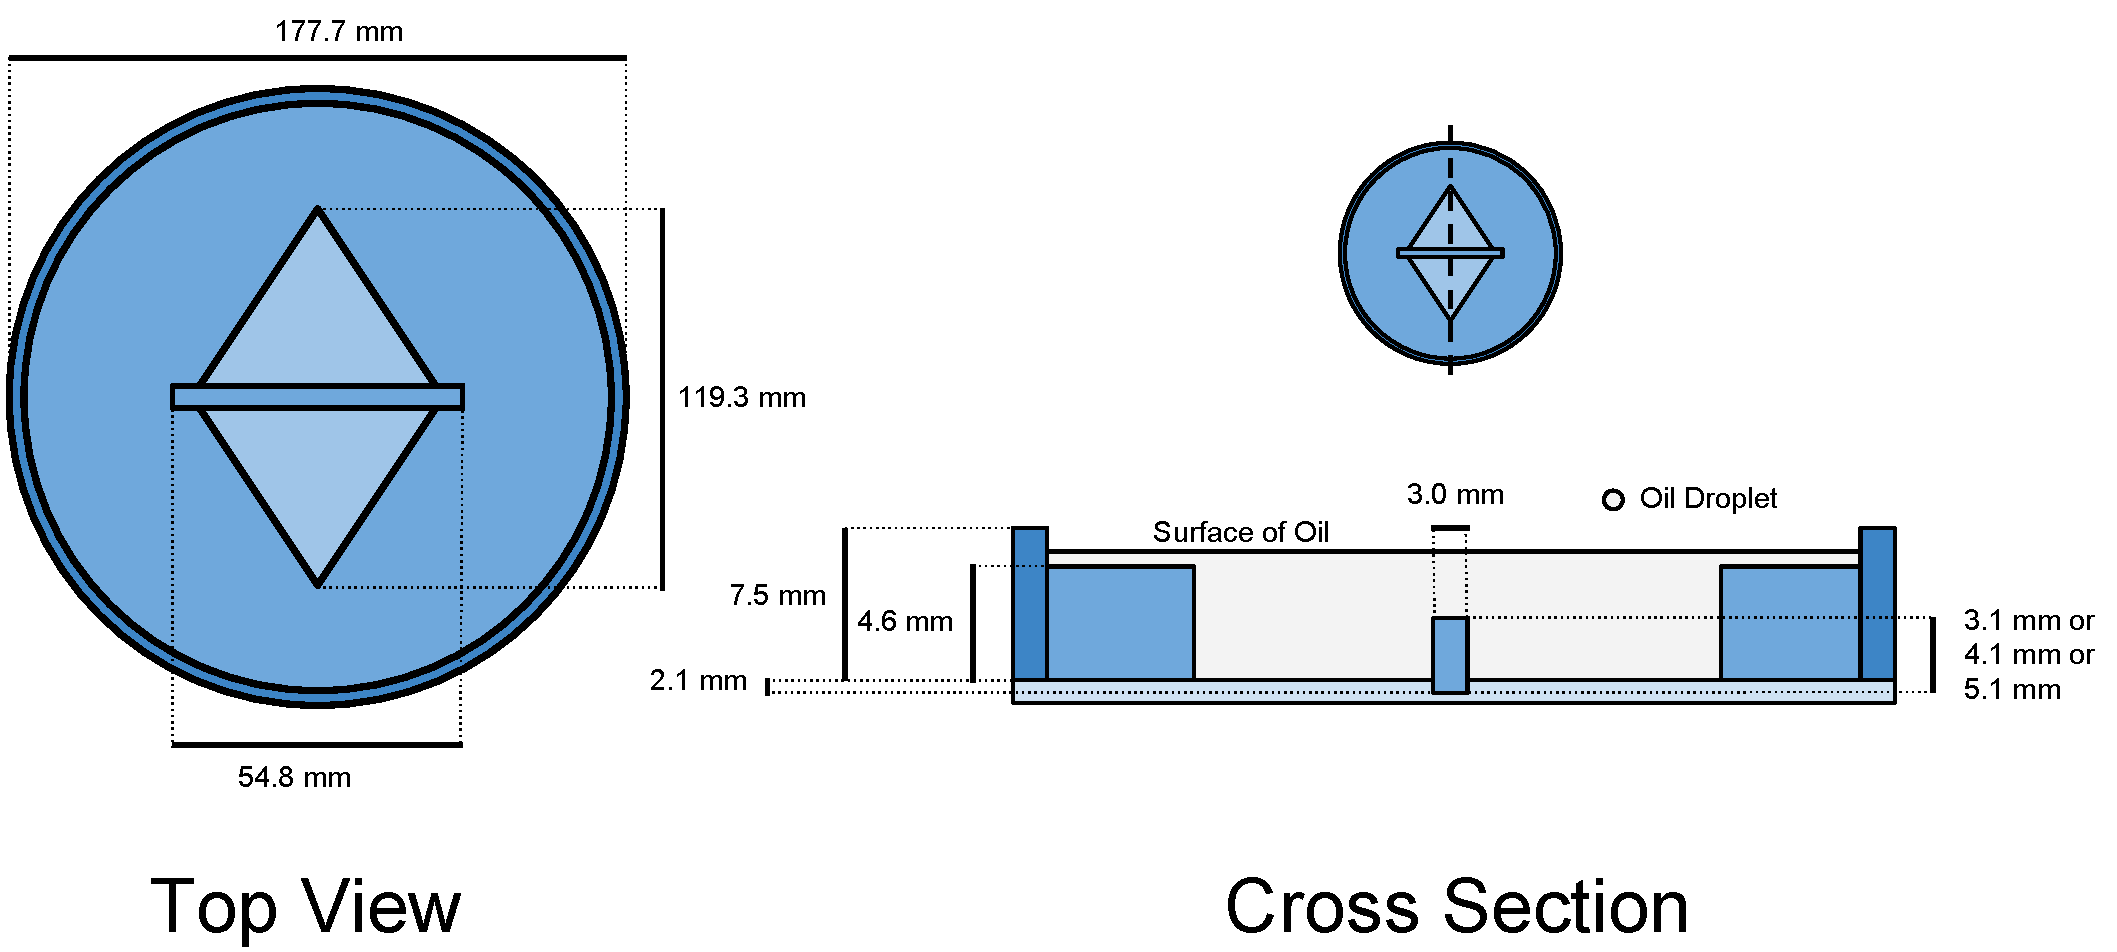
\includegraphics[scale=0.48]{Tray.pdf}
	\caption{The specifications of the tray design. The top view (left) highlights the main elements in the tray, while the cross section (right) illustrates the topography of the tray. Height is represented by the shading; darker shading is higher.}
	\label{tray}
\end{figure}

A thin layer of oil spills over the constraining rhombus shape. As long as the layer is thin enough, the droplet will remain in the rhombus container, but the waves will continue to propagate unimpeded. This gives the waves time to decay, and means that the droplets motion isn't chaotically affected by reflections of previous waves from the sidewalls, and is instead guided only by the unreflected waves. 

The rhombus shape serves to steer the droplet into a perpendicular collision with the barrier. This works because the droplet will pin-ball its way into the acute corner of the rhombus, and will shoot out in a straight line, directly towards the barrier.  (FIGURE of pinballing droplet?)

I designed my experiment to test barriers of three different heights: $2.75~\mathrm{mm}$, $3.0~\mathrm{mm}$, and $3.25~\mathrm{mm}$, measured from the bottom of the rhombus. A thin barrier of plastic made by the laser cutter has the tendency to bend and warp over time. The solution to this problem was to make these barriers taller than the specified heights, and create an cut-out in the rhombus so they could be inserted. The barrier cut-outs were deep enough to exactly counter the added height of the barrier, so the barriers still had (when measured from the surface of the rhombus) heights of $2.75~\mathrm{mm}$, $3.0~\mathrm{mm}$, and $3.25~\mathrm{mm}$. This also solved the problem of fixing the barriers in place, but still making them easily removable. These heights were chosen because they allowed for both passage over and blockage by the barriers. At the lowest heights, most droplets crossed over, whereas for taller barriers most droplets were blocked. 


The bottom of the tray was painted black in order to improve contrast, allowing the droplet to be more easily tracked by eye and by camera.

\subsection{Silicon Oil}
    Silicon oil is the ideal choice of fluid for this experiment because it remains clean, it doesn't evaporate, and it can be purchased at specific viscosities. The silicone oil used in this experiment had a viscosity of 20 cSt (its viscosity is a little closer to water than olive oil) and was purchased from Clearco Products Co. Inc., Bensalem PA (CAS No: 63148-62-9). 20 cSt silicone oil, like the one used by Bush et al.\rf{pilot-wave} was chosen because it gives a larger walking regime\rf{pilot-wave} than more viscous oil, such as the 50 cSt viscosity oil used by Couder\rf{Protiere2005}. The tray requires about $20~\mathrm{mL}$ of fluid.
    
    It is of vital importance to keep the oil as clean as possible because it keeps the droplet bouncing for longer. This means protecting from particulate matter that is already in the tray. Contamination can be minimized by cleaning the tray before pouring the oil in.
    
\subsection{Shaker}
    To shake the tray, we used a mechanical wave driver made by Pasco Scientific, Roseville CA, model SF-9324. This shaker was designed to drive a string or an elastic cord, not a $200$ gram tray with oil inside, which was probably at the limit of what the shaker can handle. 

\subsection{Waveform Generator and Amplifier}
    The shaker was driven with the Agilent Arbitrary Waveform Generator model 33210, which was controlled digitally and thus created consistent waves.  
       
    Adding a Lepai LP2020A+ digital amplifier to the wavefunction generator meant the amplitude of the tray could be precisely controlled. This signal was then fed into the shaker.    
            
\subsection{Accelerometer}  
    Knowing the tray's acceleration allows us to characterize the behavior of our system. To measure acceleration, we attached an ADLX 326 triple axis accelerometer (made by Adafruit, New York City NY) to the bottom of the tray. The method of attachment was screws, since it provided a much more firm hold than tape or glue while allowing for removal. The accelerometer has a range of $\pm$16$g$, perfect for measuring the accelerations in our setup, usually below $5g$'s. 
      
      The signal from the z-axis of the accelerometer was output directly into the oscilloscope. For the vibrating tray, the output was approximately sinusoidal (as expected). The spec sheet for the accelerometer indicates that the sensitivity can be translated to $57 \pm 6~\mathrm{mV/g}$. 
 
    
\subsection{Shield}
    A large, see-through cylinder (covered at one end) was manufactured using the laser cutter. When placed over the tray, it served the purpose of keeping the oil clean from particulate matter and preventing wind currents from influencing the motion of the walker.       
   
\subsection{Leveling Platform}
    A leveling platform was made out of wood supports the shaker. Three adjusters allowed for precise adjustment of tilt. The tray was tuned using a level placed inside the tray (before the oil was added). 

\subsection{Camera}       
 
To document trials, a Sony RX100 camera supported by a tripod aimed directly down at the tray. 

\section{Procedure}
Once the exact walking parameters are established (frequency and driving amplitude), tunneling measurements and a few different barrier heights can be made. 

\subsection{Finding the Walking Regime}

Before investigating the rate of tunneling using different barriers, a rough estimate of the walking regime at a frequency of $80~\mathrm{Hz}$ must be made. A ``map" similar to the one in \refFig{regime} will be sketched out, but rather than looking at all of the different kinds of bouncing we will limit ourselves to only the walking regime. Reproducing this figure allows us to find the parameters that are specific to our unique setup, which could have slightly different height, tray, oil, and shaker configurations than those used in the literature. 

Droplet size is measured using a recorded video of the walking droplet in motion. By comparing the number of pixels making up the diameter of the droplet (unknown measurement) to the number of pixels making up the diameter of the tray (known measurement), we can estimate the length associated with  each pixel, and thus find the diameter of the droplet in centimeters. 

Driving acceleration values are measured by the accelerometer and displayed on the oscilloscope. 

To ensure that every trial has the same oil depth, we must measure the volume of the oil before filling the tray. Knowing the volume of the tray and of each barrier, we can get a value for the oil depth without interfering with the system. In this way, oil height can be kept constant.

\subsection{The Experiment}

Tunneling was examined for three different barrier heights. At each height (and at a constant frequency of 80 Hz and constant driving acceleration), a string of continuous collisions were filmed with the camera. From this data, a basic tunneling probability was calculated, which provides the most simplistic analysis of this system. 

The tray is designed such that most of the droplet's collisions with the barrier occur ``head on" (i.e. perpendicular to the length of the barrier), but not all collisions unfold ideally. A more involved analysis in \textit{Tracker} requires looking at the component of velocity of the droplet perpendicular to the length of the barrier, and determining the probability of tunneling given this value. Since not all collisions in the simplistic analysis occur at the same velocity, this method allows for a more methodical analysis of the phenomena. 


	\chapter*{Conclusion}
         \addcontentsline{toc}{chapter}{Conclusion}
	\chaptermark{Conclusion}
	\markboth{Conclusion}{Conclusion}
	\setcounter{chapter}{4}
	\setcounter{section}{0}
	
%Here's a conclusion, demonstrating the use of all that manual incrementing and table of contents adding that has to happen if you use the starred form of the chapter command. The deal is, the chapter command in \LaTeX\ does a lot of things: it increments the chapter counter, it resets the section counter to zero, it puts the name of the chapter into the table of contents and the running headers, and probably some other stuff. 

%So, if you remove all that stuff because you don't like it to say ``Chapter 4: Conclusion'', then you have to manually add all the things \LaTeX\ would normally do for you. Maybe someday we'll write a new chapter macro that doesn't add ``Chapter X'' to the beginning of every chapter title.

The question we sought to answer was: how does tunneling probability change with the value $h$ of oil above the barrier? Our results showed that tunneling is highly sensitive in this system, and even changes in height on the order of fractions of a millimeter are enough to radically influence the proportion of tunneling droplets. Using a barrier of width $e~=~3.0~\mathrm{mm}$, it was found that a value of $h~=~1.0~\mathrm{mm}$ produced tunneling in every interaction, while for a value of $h~=~1.5~\mathrm{mm}$ there was no tunneling. In between this range was a sweet spot of $h~=~1.25~\mathrm{mm}$ where tunneling appeared probabilistic, but still somewhat dependent upon droplet diameter and droplet velocity. It would appear that for a given barrier, a droplet with a higher momentum is more likely to tunnel than a droplet with lower momentum.


The main limitations in this investigation had to do with consistency of parameters between trials, and dearth of data points. A better shaker would have significantly improved these things. The damping of the shaker we used made keeping a the same memory in every trial difficult, and limited the number trials and interactions that were filmed. The one modeled in \rf{shaker}, shakes the whole tray at the same time and with same amplitude for hours. These shakers of course, cost more than the budget allowed for, but a even conducting the tests suggested in the paper would have allowed for diagnosis of these issues. Another difficulty was in measuring the height of the oil within a trial. When removing each barrier, a certain amount of oil was lost. While this value was estimated, it still was a source of uncertainty and it introduced contamination from the pliers to get into the oil. Additionally, surely there exists a better way to measure oil depth than computing the volume of space inside the tray, but a cheap alternative was not discovered. This would have also increased uncertainty in the measurements of $h$. Using barriers of height $2.90~\mathrm{mm}$ or $3.10~\mathrm{mm}$ would have allowed for greater definition in the range of tunneling heights in \refFig{tbh}.


A few words of advice for those seeking to recreate the experiment: take your time in setting up the device, ensuring that the tray is level and that it vibrates vertically. Invest in good silicone oil, and do your best to limit any contamination of the oil. Finally, there is an accelerometer out there that does what you need it to, your task is simply to find it. 

%If you feel it necessary to include an appendix, it goes here.
	\appendix

	\chapter{The First Appendix}
An appendix full of awesome
	\chapter{The Second Appendix, for Fun}
An appendix full of win


%This is where endnotes are supposed to go, if you have them.
%I have no idea how endnotes work with LaTeX.

  \backmatter % backmatter makes the index and bibliography appear properly in the t.o.c...

% if you're using bibtex, the next line forces every entry in the bibtex file to be included
% in your bibliography, regardless of whether or not you've cited it in the thesis.
  \nocite{*}

% Rename my bibliography to be called "Works Cited" and not "References" or ``Bibliography''
% \renewcommand{\bibname}{Works Cited}

%    \bibliographystyle{bsts/mla-good} % there are a variety of styles available; 
%  \bibliographystyle{plainnat}
% replace ``plainnat'' with the style of choice. You can refer to files in the bsts or APA 
% subfolder, e.g. 
 \bibliographystyle{APA/apa-good}  % or
 \bibliography{thesis}
 % Comment the above two lines and uncomment the next line to use biblatex-chicago.
 %\printbibliography[heading=bibintoc]

% Finally, an index would go here... but it is also optional.
\end{document}
